\documentclass[20pt, a0paper, portrait]{tikzposter}

\usepackage[utf8]{inputenc}
\usepackage[T1]{fontenc}
\usepackage{textcomp}
\usepackage{arev}
\usepackage{arevmath}
\usepackage{arevtext}
\usepackage{graphicx}
\usepackage{wrapfig}
\usepackage{microtype}

% Bibliography
\usepackage[backend=biber,
bibencoding=utf8,
bibstyle=numeric-comp,
%style=verbose, %verbose-ibid,
url=true, % include url in reference
doi=true, % include doi in reference
sorting=none, % sorting of citations
%autocite=superscript, % autocite becomes superscript
maxcitenames=1, % Max names displayed when citing in text
maxbibnames=10, % Max number of names displayed in the bibliography
giveninits=true % Use initials
]{biblatex}
\addbibresource{citations.bib}
\renewcommand*{\bibfont}{\footnotesize}

\renewcommand*\familydefault{\sfdefault}

\title{Engineering Design}
\author{Engineering Design \& Manufacture Group}
\date{\today}
\institute{University of Bath, UK}

\usetheme{Default}
\usecolorstyle[colorPalette=GreenGrayViolet]{Default}
\useblockstyle{Default}
\usetitlestyle{Filled}

\begin{document}

\maketitle

\begin{columns}
  \column{0.5}
    \block[]{Introduction}{
      Engineering Design is the discipline of transferring your theoretical knowledge and understanding of engineering systems into practical and usable products. You may find it interesting to discover that up to 80\% of the committed cost of a product occurs when decisions are made early-on in its design (Figure~\ref{fig-committed}).~\autocite{ullman2002}~\autocite{corbett1986}~\autocite{mileham1993}

      \begin{tikzfigure}[The committed cost during a design project~\autocite{ullman2002}]
        \centering
        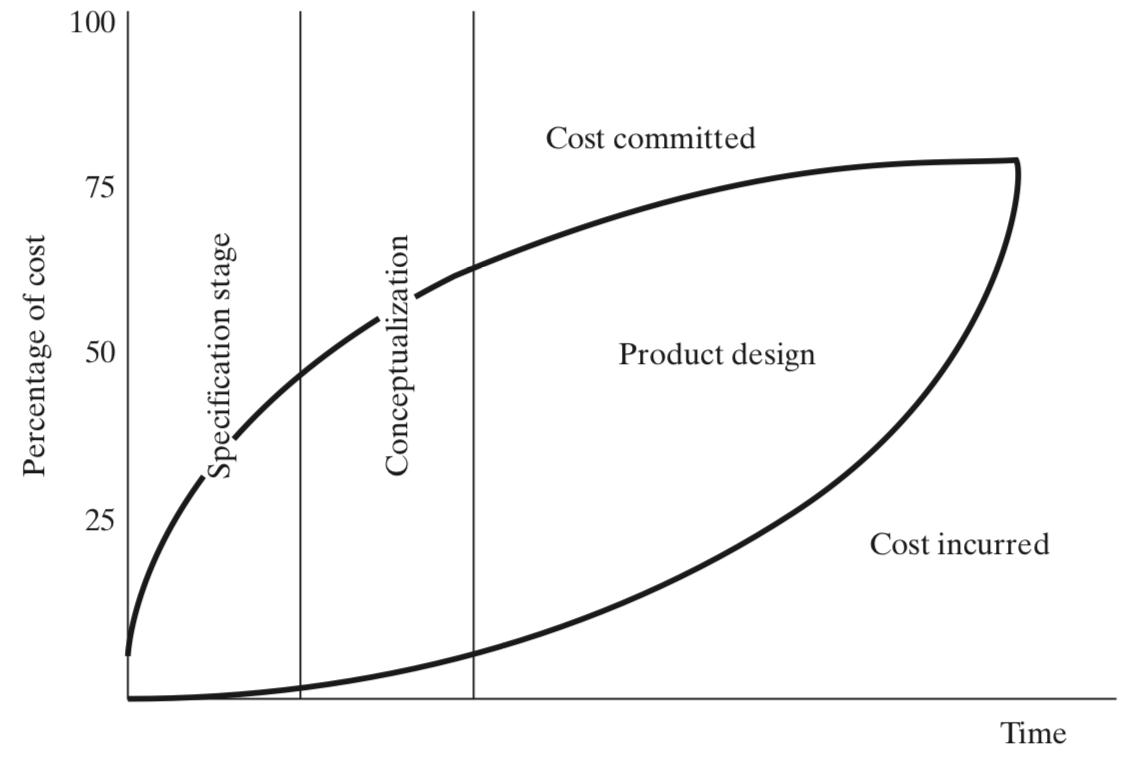
\includegraphics[width=0.3\textwidth]{commited-cost.png}
        \label{fig-committed}
      \end{tikzfigure}

      It is the objective of the designer to consider all the potential implications of these decisions and their impact across the Product's Lifecycle. This is becoming evermore critical as companies become more reliant on the sale of products as part of a service, which is often referred to as Product Service Systems. For example, Rolls-Royce's sale strategy is now focused on the idea of `Power by the Hour'. Thus, issues in the design of the product can greatly impact the profitability and safety of the service they provide.

      With companies becoming ever-more global, engineering teams are often collaborating across the world on new product development. The competencies and skills that you will develop throughout your design exercises in Bath will enable you to meet these challenges head-on.

      \textbf{33\%} It may also be interesting to know that the majority of you will progress into higher-levels of management, be it in an engineering, consultancy, medical, banking, start-up and/or other industrial sectors. The success of engineers in business is further demonstrated by the fact that a third of the top CEO's have an engineering degree.~\autocite{bi2011}~\autocite{hbr2014} Nearly as many who have an MBA! 

      The reason for this has been attributed to how we define, manage, communicate, structure and solve problems in teams, and this is what Engineering Design is all about!
    }
  \column{0.5}

  \block[]{References}{
    \printbibliography[heading=none]{}
  }
\end{columns}

\end{document}